\chapter{Esempio di capitolo} %\label{1cap:spinta_laterale}

\begin{preamble}
{\em Riassunto del capitolo. In questo capitolo...}
\end{preamble}

\section{Sezione 1}
Sezione 1 del capitolo con Figura \ref{fig:esempio}

\begin{figure}[h]
	\centering
	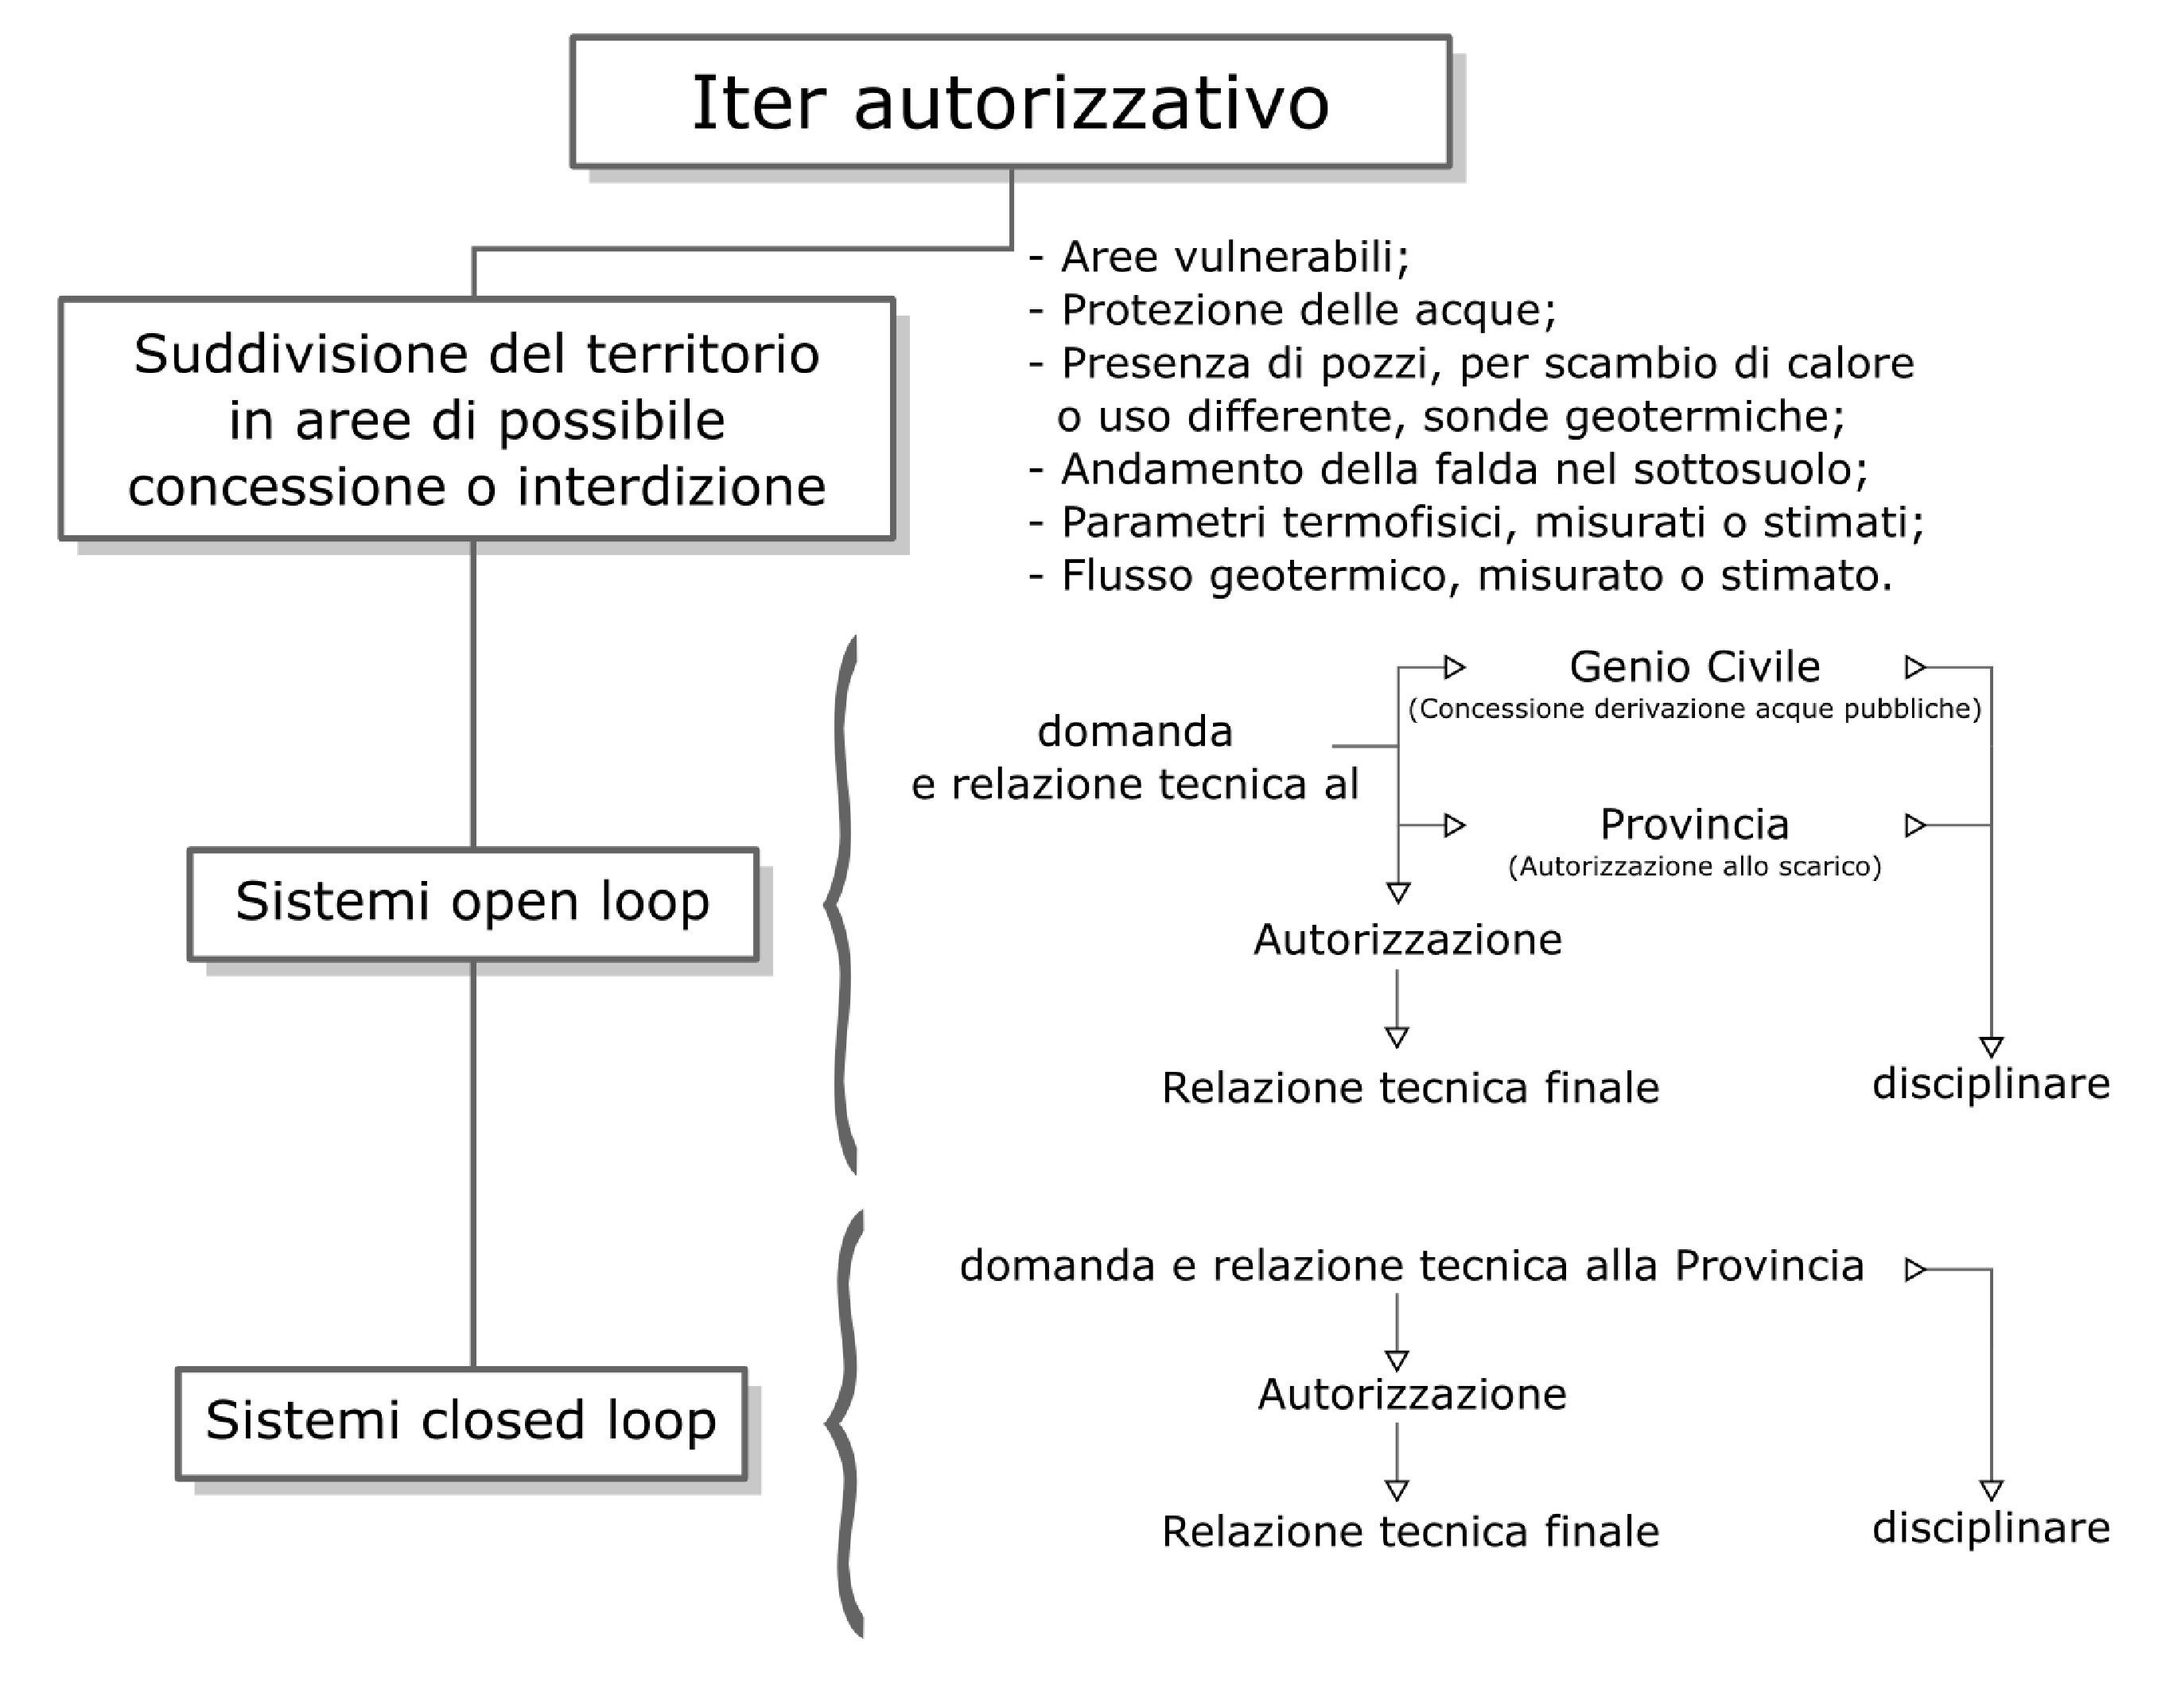
\includegraphics [width=.95\columnwidth, angle=0]{iter_autorizzativo} % height
	\caption{Figura Esempio}
	\label{fig:esempio}
\end{figure}

\subsection{Sezione 2}
Sezione 2 con sottosezione.

\subsection{Sottosezione 2.1}
Sottosezione con Tabella \ref{tab:esempio}.

\begin{table}[h]
\centering
\rowcolors{2}{gray!25}{}
\begin{tabular}{lll}
\toprule
{\bf Valore 1} & {\bf Valore 2} & {\bf Valore 3} \\
\midrule
10	& 20 & 30 \\
40 & 50 & 60 \\
\bottomrule
\end{tabular}
\caption{Tabella di esempio}
\label{tab:esempio}
\end{table}